% \begin{frame}{Genus sumy spójnej}{obrazek dowodu $g(K_1\# K_2) \geq g(K_1)+g(K_2)$}
%   \begin{center}
%     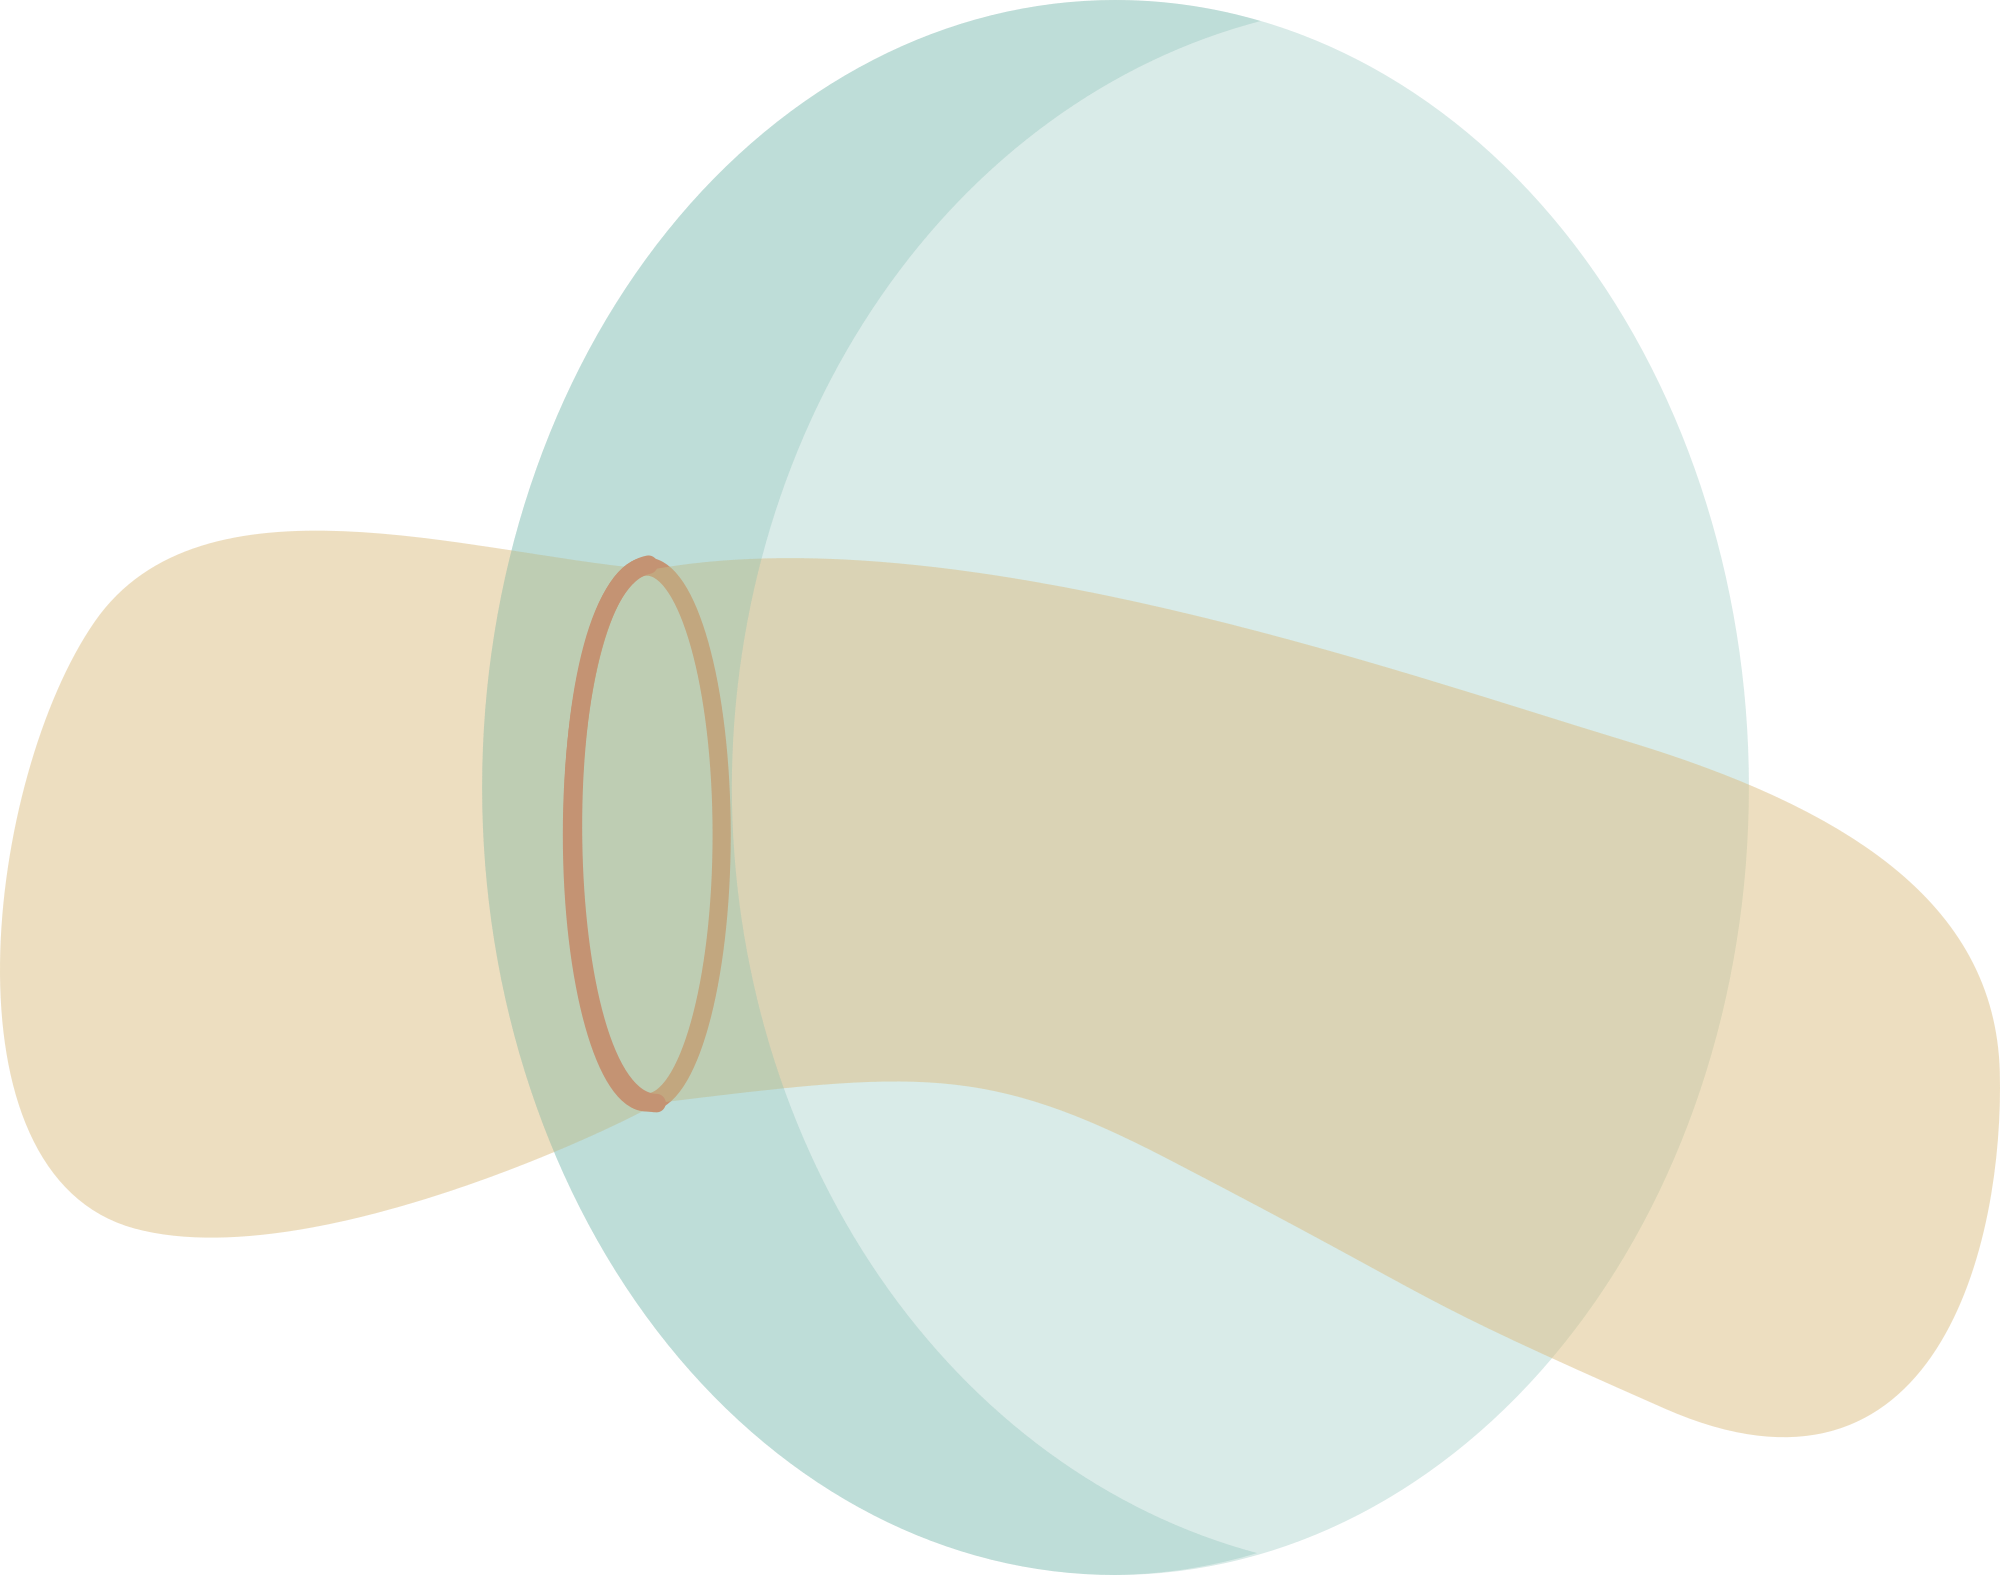
\includegraphics[width=0.9\textheight]{rysunek-dowod-suma-spojna.png}
%   \end{center}
% \end{frame}

\begin{frame}{Genus sumy spójnej}{dowód $g(K_1\# K_2) \geq g(K_1)+g(K_2)$}
  \begin{itemize}
    \item Zaczynamy od powierzchni $F$ minimalizującej genus $K_1\# K_2$.

    \item Niech $S$ będzie $2$-sferą rozdzielającą $K_1$ od $K_2$, które przecina $F$ tak, że $S\cap F$ to suma okręgów niebrzegowych i jednego łuczku między dwoma punktami $S\cap K$.
    \item Na $S$ widzimy $n$ okręgów przychodzących z $S\cap F$. Rozcinając $S$ wzdłuż nich wszystkich dostajemy $n$ powierzchni $C_1,..., C_n$ takich, że 
      $$2=\chi(S)=\sum_{i=1}^n\chi(C_i)$$
      czyli istnieje $i$ takie, że $\chi(C_i)>0$.
  \end{itemize}
\end{frame}

\begin{frame}{Genus sumy spójnej}{ciąg dalszy dowodu $g(K_1\# K_2) \geq g(K_1)+g(K_2)$}
  \begin{itemize}
    \item Niech $C$ będzie rozmaitością powstałą przez rozcięcie dla której $\chi(C)>0$.
    \item $\chi(C)=2-2g-b$, gdzie $b$ to ilość komponent brzegu. Zarówno $g,b\geq 0$, więc $\chi(C)=2$ czyli $C$ to dyszczek.
    \item Rozcinamy $F$ wzdłuż brzegu $C$ i zaklejamy krwawiące końce dwoma dyszczkami by dostać $F'$. Gdybyśmy w ten sposób nadal mieli jedną rozmaitość w ręku, to 
      \begin{center}
        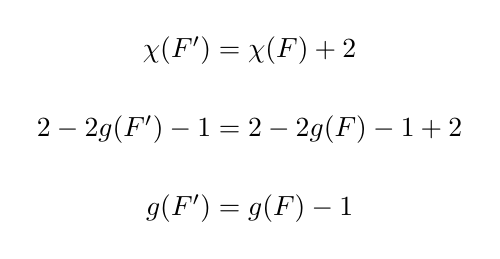
\begin{tikzpicture}
          \node at (0,0) {$\chi(F')=\chi(F)+2$};
          \node at (0, -1) {$2-2g(F')-1=2-2g(F)-1+2$};
          \node at (0, -2) {$g(F')=g(F)-1$};
          \node[rotate=-90] at (0, -0.5) {$\implies$};
          \node[rotate=-90] at (0, -1.5) {$\implies$};
        \end{tikzpicture}
      \end{center}
      co daje sprzeczność z minimalnością $g(F)$.
  \end{itemize}
\end{frame}

\begin{frame}{Genus sumy spójnej}{ciąg dalszy ciągu dalszego dowodu $g(K_1\# K_2)\geq g(K_1)+g(K_2)$}
  \begin{itemize}
    \item Po rozcięciu dostajemy więc dwie rozmaitości: $F'=F''+X$. Wiemy, że 
      $$\chi(F)+2=\chi(F')=\chi(F'')+\chi(X).$$
    \item Rozcinając i wklejając dyszczki nie zmieniliśmy brzegu $F'$, więc $F''$ nadal ma jedną komponentę spójności a $X$ jest zamknięte.
    \item Wiemy więc, że $\chi(X)\leq 2$, a łącząc to z faktem, że $X$ jest zamkniętą powierzchnią wiemy, że $X=S^2$ i $\chi(X)=2$.
  \end{itemize}
\end{frame}

\begin{frame}{Genus sumy spójnej}{koniec ciągu dalszego dowodu $g(K_1\# K_2)\geq g(K_1)+g(K_2)$}
  \begin{itemize}
    \item W takim razie $\chi(F'')=\chi(F)$ i dzielą one również genus.
    \item Powtarzamy historię aż przekrój będzie miał tylko łuczek między dwoma punktami $S\cap K$.
    \item Wtedy umiemy rozciąć nową powierzchnię $F$ rzeczonym łuczkiem, by dostać dwie powierzchnie $F_1$ i $F_2$, których brzegi to odpowiedni $K_1$ i $K_2$.
    \item Po cichu dokleiliśmy kreseczkę, więc
      $$\chi(F)=\chi(F_1)+\chi(F_2)-\chi(\kreska)$$
      $$g(K_1)+g(K_2)\leq g(F_1)+g(F_2)=g(F).$$
  \end{itemize}

  \begin{tikzpicture}[overlay, remember picture]
    \node at (\paperwidth/6 * 5,0) {
\includegraphics[width=1cm]{../Donald_Duck.png}};
  \end{tikzpicture}
\end{frame}
